\documentclass[tikz,border=5pt]{standalone}
\usepackage{tikz}
\usetikzlibrary{positioning,shapes.geometric,arrows.meta,fit,calc}

\definecolor{inputcolor}{RGB}{240,240,240}
\definecolor{convcolor}{RGB}{232,245,232}
\definecolor{densecolor}{RGB}{227,242,253}
\definecolor{attentioncolor}{RGB}{243,229,245}

\begin{document}
	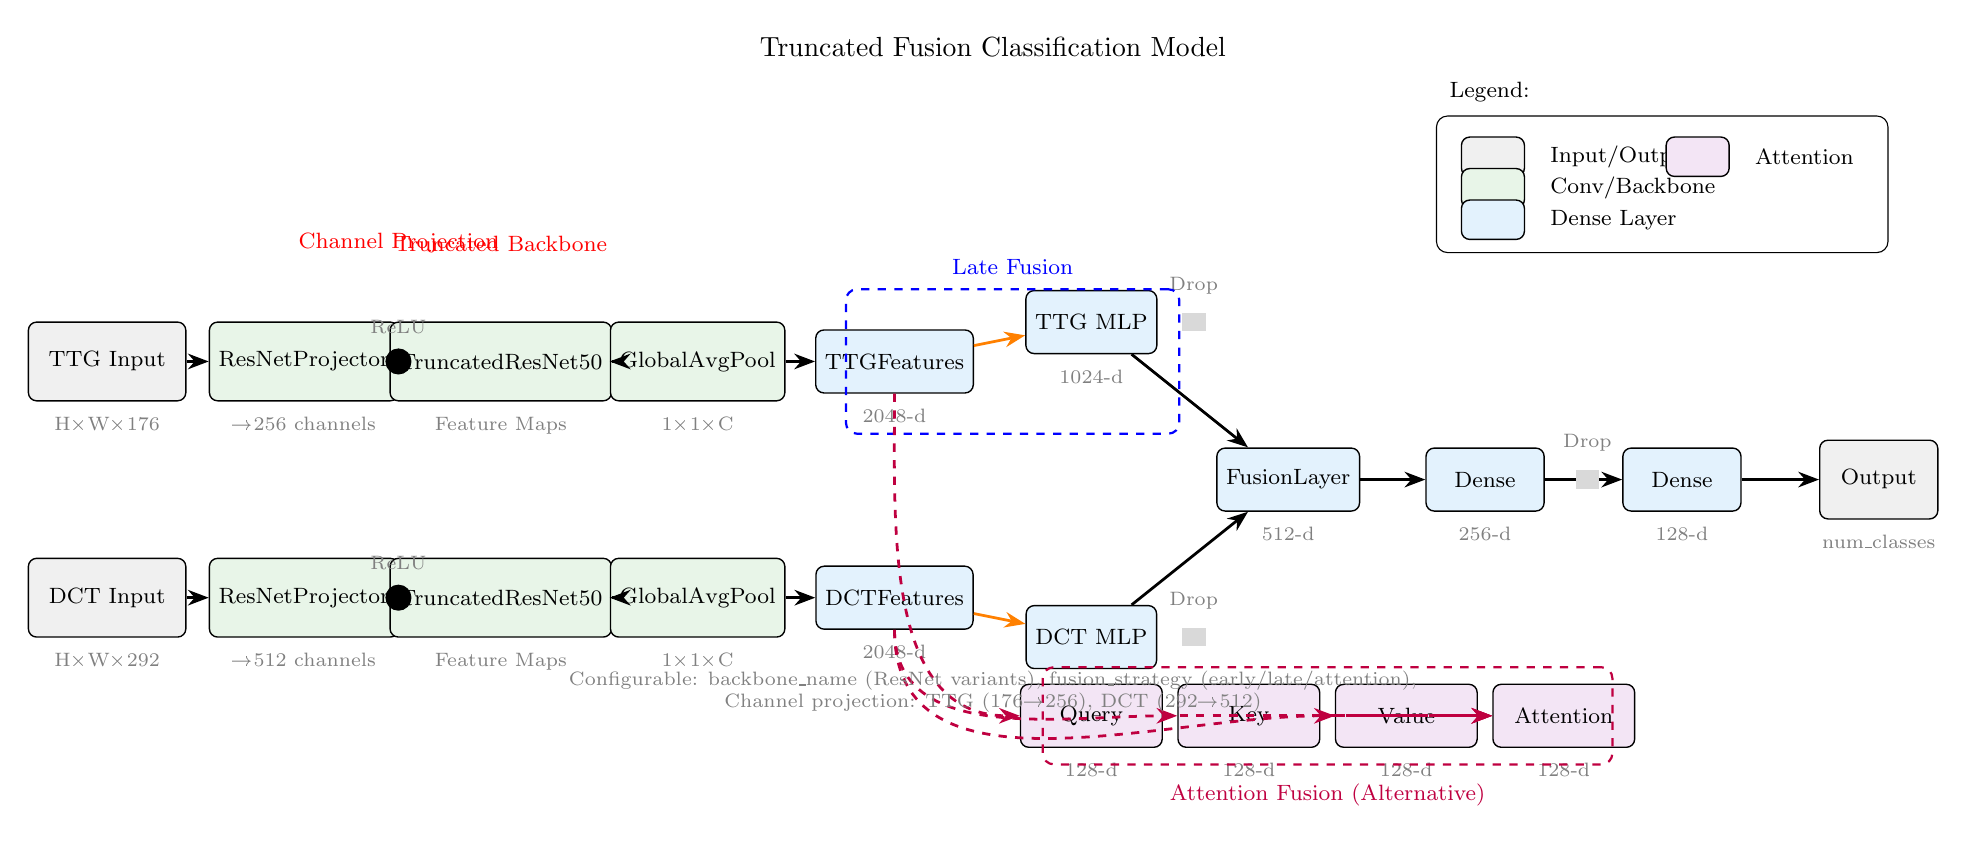
\begin{tikzpicture}[
		% Layer styles
		input/.style={rectangle, rounded corners=3pt, minimum height=1cm, minimum width=2cm, 
			fill=inputcolor, draw=black, line width=0.5pt, text centered, font=\footnotesize},
		conv/.style={rectangle, rounded corners=3pt, minimum height=1cm, minimum width=1.8cm,
			fill=convcolor, draw=black, line width=0.5pt, text centered, font=\footnotesize},
		dense/.style={rectangle, rounded corners=3pt, minimum height=0.8cm, minimum width=1.5cm,
			fill=densecolor, draw=black, line width=0.5pt, text centered, font=\footnotesize},
		attention/.style={rectangle, rounded corners=3pt, minimum height=0.8cm, minimum width=1.8cm,
			fill=attentioncolor, draw=black, line width=0.5pt, text centered, font=\footnotesize},
		output/.style={rectangle, rounded corners=3pt, minimum height=1cm, minimum width=1.5cm,
			fill=inputcolor, draw=black, line width=0.5pt, text centered, font=\footnotesize},
		% Arrow styles
		arrow/.style={->, >=Stealth, thick, line width=1pt},
		fusionarrow/.style={->, >=Stealth, thick, line width=1pt, color=orange},
		attnarrow/.style={->, >=Stealth, thick, line width=1pt, dashed, color=purple},
		% Text styles
		dimlabel/.style={font=\scriptsize, text=gray},
		layerlabel/.style={font=\footnotesize}
		]
		
		% Input layers
		\node[input] (ttg_input) at (0,5) {TTG Input};
		\node[dimlabel, below=2pt of ttg_input] {H×W×176};
		
		\node[input] (dct_input) at (0,2) {DCT Input};
		\node[dimlabel, below=2pt of dct_input] {H×W×292};
		
		% Channel projection layers
		\node[conv] (ttg_proj) at (2.5,5) {ResNet\\Projector};
		\node[dimlabel, below=2pt of ttg_proj] {→256 channels};
		
		\node[conv] (dct_proj) at (2.5,2) {ResNet\\Projector};
		\node[dimlabel, below=2pt of dct_proj] {→512 channels};
		
		% Truncated backbone networks
		\node[conv] (ttg_backbone) at (5,5) {Truncated\\ResNet50};
		\node[dimlabel, below=2pt of ttg_backbone] {Feature Maps};
		
		\node[conv] (dct_backbone) at (5,2) {Truncated\\ResNet50};
		\node[dimlabel, below=2pt of dct_backbone] {Feature Maps};
		
		% Global Average Pooling
		\node[conv] (ttg_pool) at (7.5,5) {Global\\AvgPool};
		\node[dimlabel, below=2pt of ttg_pool] {1×1×C};
		
		\node[conv] (dct_pool) at (7.5,2) {Global\\AvgPool};
		\node[dimlabel, below=2pt of dct_pool] {1×1×C};
		
		% Feature vectors after flattening
		\node[dense] (ttg_features) at (10,5) {TTG\\Features};
		\node[dimlabel, below=2pt of ttg_features] {2048-d};
		
		\node[dense] (dct_features) at (10,2) {DCT\\Features};
		\node[dimlabel, below=2pt of dct_features] {2048-d};
		
		% Fusion strategies (showing late fusion as default)
		\node[dense] (ttg_mlp) at (12.5,5.5) {TTG MLP};
		\node[dimlabel, below=2pt of ttg_mlp] {1024-d};
		
		\node[dense] (dct_mlp) at (12.5,1.5) {DCT MLP};
		\node[dimlabel, below=2pt of dct_mlp] {1024-d};
		
		% Concatenation and fusion
		\node[dense] (fusion) at (15,3.5) {Fusion\\Layer};
		\node[dimlabel, below=2pt of fusion] {512-d};
		
		% Final classifier
		\node[dense] (classifier1) at (17.5,3.5) {Dense};
		\node[dimlabel, below=2pt of classifier1] {256-d};
		
		\node[dense] (classifier2) at (20,3.5) {Dense};
		\node[dimlabel, below=2pt of classifier2] {128-d};
		
		\node[output] (final_output) at (22.5,3.5) {Output};
		\node[dimlabel, below=2pt of final_output] {num\_classes};
		
		% Main data flow arrows
		\draw[arrow] (ttg_input) -- (ttg_proj);
		\draw[arrow] (dct_input) -- (dct_proj);
		\draw[arrow] (ttg_proj) -- (ttg_backbone);
		\draw[arrow] (dct_proj) -- (dct_backbone);
		\draw[arrow] (ttg_backbone) -- (ttg_pool);
		\draw[arrow] (dct_backbone) -- (dct_pool);
		\draw[arrow] (ttg_pool) -- (ttg_features);
		\draw[arrow] (dct_pool) -- (dct_features);
		
		% Fusion pathway
		\draw[fusionarrow] (ttg_features) -- (ttg_mlp);
		\draw[fusionarrow] (dct_features) -- (dct_mlp);
		\draw[arrow] (ttg_mlp) -- (fusion);
		\draw[arrow] (dct_mlp) -- (fusion);
		
		% Classification pathway
		\draw[arrow] (fusion) -- (classifier1);
		\draw[arrow] (classifier1) -- (classifier2);
		\draw[arrow] (classifier2) -- (final_output);
		
		% Activation functions (ReLU indicators)
		\node[circle, fill=black, minimum size=3pt] at (3.7,5) {};
		\node[dimlabel, above=1pt] at (3.7,5.2) {ReLU};
		
		\node[circle, fill=black, minimum size=3pt] at (3.7,2) {};
		\node[dimlabel, above=1pt] at (3.7,2.2) {ReLU};
		
		% Dropout indicators
		\node[rectangle, minimum width=0.3cm, minimum height=0.1cm, fill=gray!30] at (13.8,5.5) {};
		\node[dimlabel, above=1pt] at (13.8,5.7) {Drop};
		
		\node[rectangle, minimum width=0.3cm, minimum height=0.1cm, fill=gray!30] at (13.8,1.5) {};
		\node[dimlabel, above=1pt] at (13.8,1.7) {Drop};
		
		\node[rectangle, minimum width=0.3cm, minimum height=0.1cm, fill=gray!30] at (18.8,3.5) {};
		\node[dimlabel, above=1pt] at (18.8,3.7) {Drop};
		
		% Alternative fusion strategies (shown with dashed boxes)
		% Early fusion alternative
		\node[draw, dashed, rounded corners, fit={(9.5,4.2) (13.5,5.8)}, color=blue, line width=0.8pt] {};
		\node[layerlabel, color=blue] at (11.5,6.2) {Late Fusion};
		
		% Attention fusion alternative (shown below)
		\node[attention] (query_proj) at (12.5,0.5) {Query};
		\node[dimlabel, below=2pt of query_proj] {128-d};
		\node[attention] (key_proj) at (14.5,0.5) {Key};
		\node[dimlabel, below=2pt of key_proj] {128-d};
		\node[attention] (value_proj) at (16.5,0.5) {Value};
		\node[dimlabel, below=2pt of value_proj] {128-d};
		\node[attention] (multihead_attn) at (18.5,0.5) {Attention};
		\node[dimlabel, below=2pt of multihead_attn] {128-d};
		
		\draw[attnarrow] (ttg_features.south) to[out=-90,in=180] (query_proj.west);
		\draw[attnarrow] (dct_features.south) to[out=-90,in=180] (key_proj.west);
		\draw[attnarrow] (dct_features.south) to[out=-90,in=180] (value_proj.west);
		\draw[attnarrow] (query_proj) -- (multihead_attn);
		\draw[attnarrow] (key_proj) -- (multihead_attn);
		\draw[attnarrow] (value_proj) -- (multihead_attn);
		
		\node[draw, dashed, rounded corners, fit={(12,0) (19,1)}, color=purple, line width=0.8pt] {};
		\node[layerlabel, color=purple] at (15.5,-0.5) {Attention Fusion (Alternative)};
		
		% Legend
		\node[draw, rounded corners, fit={(17,6.5) (22.5,8)}, fill=white] (legend) {};
		\node[layerlabel, above right=2pt of legend.north west] {Legend:};
		\node[input, minimum width=0.8cm, minimum height=0.5cm] at (17.6,7.6) {};
		\node[layerlabel, right=3pt] at (18.1,7.6) {Input/Output};
		\node[conv, minimum width=0.8cm, minimum height=0.5cm] at (17.6,7.2) {};
		\node[layerlabel, right=3pt] at (18.1,7.2) {Conv/Backbone};
		\node[dense, minimum width=0.8cm, minimum height=0.5cm] at (17.6,6.8) {};
		\node[layerlabel, right=3pt] at (18.1,6.8) {Dense Layer};
		\node[attention, minimum width=0.8cm, minimum height=0.5cm] at (20.2,7.6) {};
		\node[layerlabel, right=3pt] at (20.7,7.6) {Attention};
		
		% Key innovation annotation
		\node[layerlabel, color=red, font=\footnotesize] at (3.7,6.5) {Channel Projection};
		\node[layerlabel, color=red, font=\footnotesize] at (5,6.5) {Truncated Backbone};
		
		% Title
		\node[layerlabel, font=\normalsize] at (11.25,9) {Truncated Fusion Classification Model};
		
		% Configuration note
		\node[layerlabel, font=\scriptsize, text=gray] at (11.25,0.8) {
			\begin{tabular}{c}
				Configurable: backbone\_name (ResNet variants), fusion\_strategy (early/late/attention), \\
				Channel projection: TTG (176→256), DCT (292→512)
		\end{tabular}};
		
	\end{tikzpicture}
\end{document}